\documentclass[10pt]{article}
\usepackage[utf8]{inputenc}
\usepackage[T1]{fontenc}
\usepackage{lmodern}
\usepackage[letterpaper,margin=0.66in]{geometry}
\usepackage{microtype}
\usepackage{amsmath,amssymb}
\usepackage{graphicx}
\usepackage{booktabs}
\usepackage{siunitx}
\usepackage{xcolor}
\usepackage[hidelinks]{hyperref}
\hypersetup{
  pdftitle={Connecting the Dots in AMR Surveillance},
  pdfauthor={Giordano De Marzo, Alfredo De Bellis, Chiara Mastrogiuseppe},
  pdfsubject={Vivli AMR Surveillance Data Challenge final report}
}
\usepackage[font=footnotesize,labelfont=bf]{caption}
\usepackage{enumitem}
\usepackage{titlesec}
\usepackage{float}
\usepackage{array}
\usepackage{multicol}

\definecolor{navy}{HTML}{17324D}
\definecolor{teal}{HTML}{246B70}
\setlength{\parindent}{0pt}
\setlength{\parskip}{3.5pt}
\setlength{\textfloatsep}{5pt}
\setlength{\floatsep}{5pt}
\setlength{\intextsep}{5pt}
\setlength{\abovecaptionskip}{3pt}
\setlength{\belowcaptionskip}{0pt}
\setlist{nosep,leftmargin=1.35em}
\titleformat{\section}{\large\bfseries\color{navy}}{}{0pt}{}
\titleformat{\subsection}{\normalsize\bfseries\color{teal}}{}{0pt}{}
\titlespacing*{\section}{0pt}{6pt}{2pt}
\titlespacing*{\subsection}{0pt}{4pt}{1pt}
\newcommand{\rca}{\mathrm{RCA}}
\newcommand{\N}{\mathcal{N}}
\newcommand{\I}{\mathcal{I}}
\newcommand{\E}{\mathcal{E}}

\begin{document}

\begin{center}
{\LARGE\bfseries\color{navy} Connecting the Dots in AMR Surveillance}\par
\vspace{1pt}
{\large\color{teal} An interpretable network framework for structure, ranking and prospective prioritisation}\par
\vspace{4pt}
{\normalsize Giordano De Marzo, Alfredo De Bellis, Chiara Mastrogiuseppe}\par
\end{center}
\vspace{-3pt}

\section*{Abstract}
Routine antimicrobial-resistance (AMR) surveillance is commonly summarised one pathogen--antibiotic pair at a time, leaving the joint structure of resistance profiles largely unused. We present a transparent framework that converts surveillance counts into a bipartite network of pathogen--antibiotic links that are comparatively prominent within the selected dataset. The network is used to test whether the surveillance landscape contains one global hierarchy or several local ones, to derive context-specific pathogen and antibiotic rankings, and to prospectively prioritise links that become comparatively prominent in the following year. Applied to Pfizer ATLAS data accessed through the Vivli AMR Register, the RCA-positive matrix contained locally ordered modules rather than a single global ladder. Rankings computed within these modules showed external consistency with WHO AWaRe tiers and ESKAPEE groupings, and a simple network-exposure score discriminated next-year RCA-positive transitions in rolling-origin evaluation. Every output follows an explicit path from isolate counts to a traceable score, without fitting a black-box classifier. The framework complements pairwise surveillance with a reproducible relational view that can be re-estimated across time and, after isolate-level re-aggregation, across geography.

\section*{Objectives}
Pairwise percentages answer how much resistance was observed for a specific pathogen and antibiotic, but not how that pair sits within the wider surveillance landscape. We therefore pursued three linked objectives: (i) construct an interpretable network of within-dataset comparative-resistance signals; (ii) determine whether the network's organisation supports meaningful local rankings of pathogens and antibiotics; and (iii) test prospectively whether proximity to existing signals can prioritise the pairs that become comparatively prominent in the next year.

\section*{Methods}
\subsection*{Data, resistance fractions and revealed comparative resistance}
The input contains annual species--antibiotic counts from the Pfizer ATLAS surveillance programme distributed through Vivli, spanning 394 species, 43 antibiotics and 2004--2024. For every analysis window, resistant and tested counts were first pooled. A pair $(p,a)$ was retained only when at least 30 isolates had been tested, and its resistance fraction was
\[
 r_{pa}=\frac{n^R_{pa}}{N_{pa}},
\]
where intermediate isolates contribute to $N_{pa}$ but not to $n^R_{pa}$. If the pair was absent or did not reach the threshold, $r_{pa}$ was undefined.

Raw percentages are difficult to compare across a heterogeneous table: some pathogens have broadly high resistance fractions, while some antibiotics have high resistance fractions across many pathogens. We therefore adapted revealed comparative advantage from Economic Complexity~\cite{hidalgo2009,tacchella2012}. Let $\mathcal O$ be the observed cells in a window, $R_p=\sum_{a:(p,a)\in\mathcal O}r_{pa}$, $A_a=\sum_{p:(p,a)\in\mathcal O}r_{pa}$ and $T=\sum_{(p,a)\in\mathcal O}r_{pa}$. Then
\[
 \rca_{pa}=\frac{r_{pa}}{R_pA_a/T}=\frac{r_{pa}T}{R_pA_a}.
\]
Thus $\rca_{pa}\geq1$ identifies a resistance fraction at least as large as the value implied by the pathogen and antibiotic marginals in that same dataset and time window; for example, $\rca_{pa}=2$ denotes twice that marginal expectation. We call this an \emph{RCA-positive} or \emph{revealed comparative-resistance} link; it is not a clinical breakpoint or an absolute biological label. The implemented binary matrix is
\[
 M_{pa}=\mathbf 1\{\rca_{pa}\geq1\}.
\]
Because comparisons with undefined RCA evaluate as false in the pipeline, $M_{pa}=0$ combines observed cells with $\rca_{pa}<1$ and insufficiently observed cells. A zero therefore means ``no RCA-positive link in the analysed surveillance universe'', not confirmed susceptibility.



\newpage
\section*{Methods (continued)}
\begin{figure}[H]
\centering
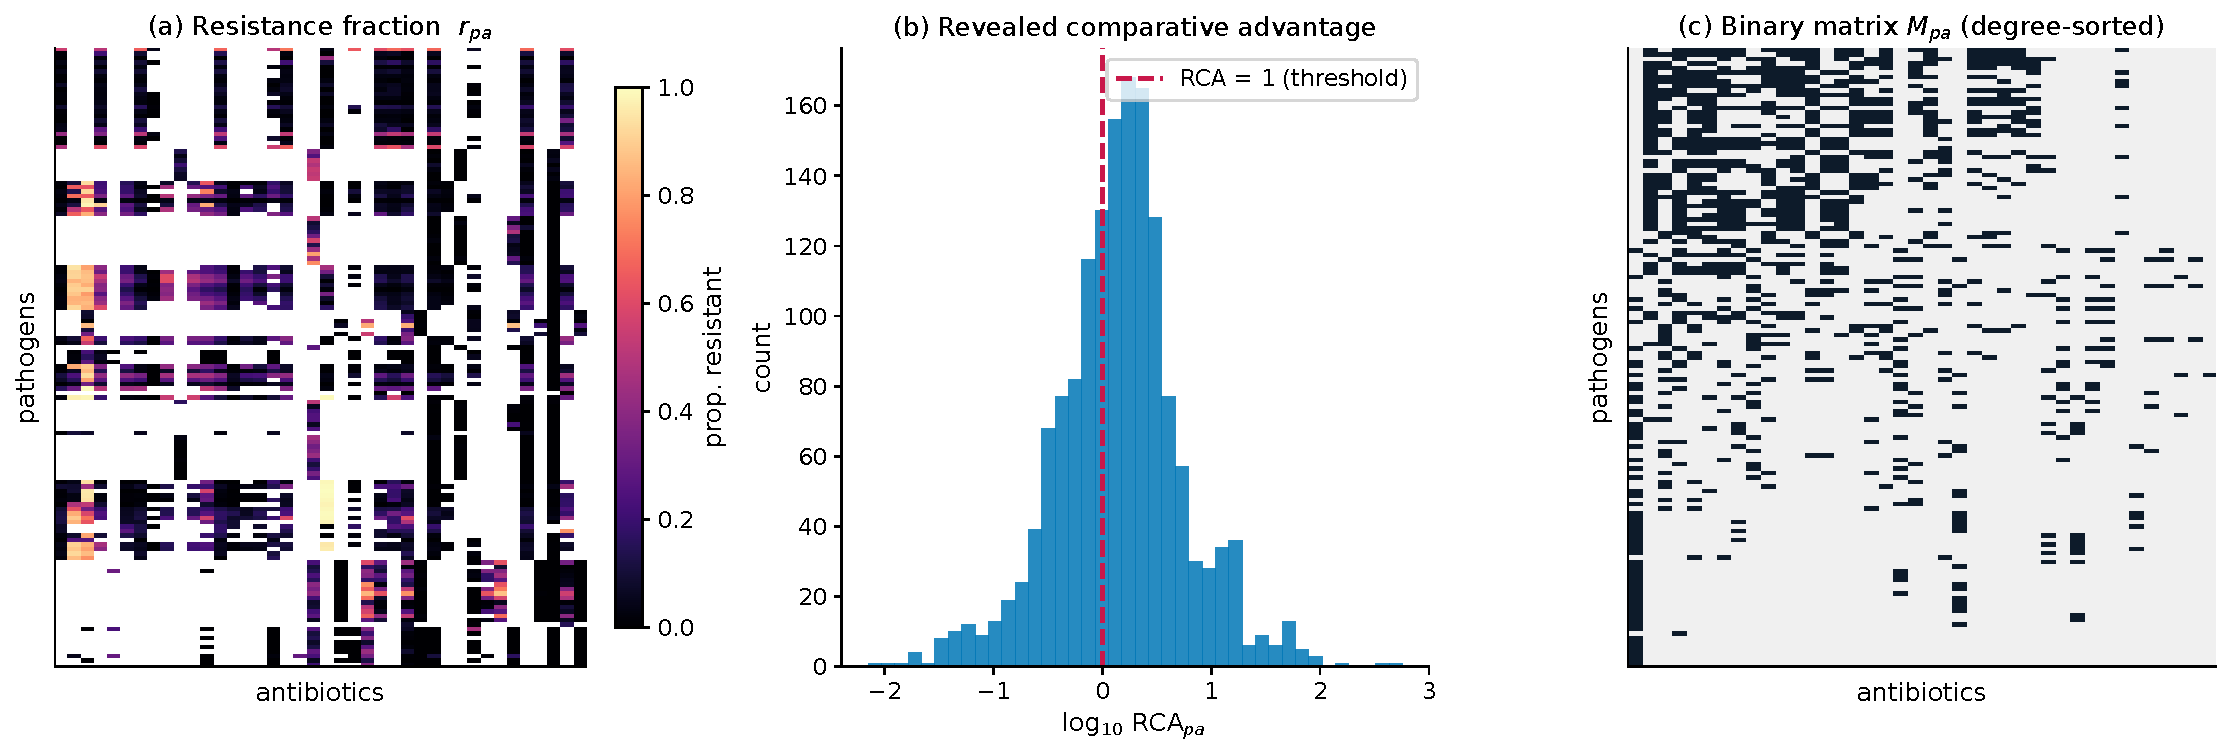
\includegraphics[width=0.82\textwidth]{figures/fig1_binarization.pdf}
\caption{From surveillance counts to the bipartite network. Pooled resistance fractions (a) are normalised into RCA values (b) and thresholded at $\rca=1$ to obtain $M$ (c). RCA defines a within-dataset comparative signal, not a clinical susceptibility category.}
\end{figure}
\vspace{-2pt}
\begin{multicols}{2}
\small
\subsection*{Why measure nestedness?}
Economic Complexity was developed for country--product networks. In a globally nested export matrix, less diversified countries tend to export subsets of the products exported by more diversified countries, while uncommon products occur mainly in diversified economies. After sorting rows and columns by degree, this produces one approximately triangular hierarchy. We asked whether the RCA-positive AMR matrix has an analogous subset ordering: do narrower pathogen profiles sit inside broader profiles, and do antibiotics linked to fewer pathogens occur within the sets linked to more pathogens?

For two row nodes $i,j$, let $k_i$ and $k_j$ be their degrees and $O_{ij}=\sum_aM_{ia}M_{ja}$ their number of shared neighbours. Under a degree-based expectation, $\langle O_{ij}\rangle=k_ik_j/A$, where $A$ is the number of antibiotic columns. The row contribution compares the excess overlap of a lower-degree node with a higher-degree node, normalised by the maximum possible overlap. An analogous term is computed for columns. The implemented in-block score is~\cite{soleribalta2018,laudati2023}
\[
\begin{aligned}
\I_R&=\sum_{\substack{i,j\\ k_i>k_j,\,b_i=b_j}}
\frac{O_{ij}-k_ik_j/A}{k_j(C_i-1)},\\[-1pt]
\I_C&=\sum_{\substack{a,c\\ k_a>k_c,\,b_a=b_c}}
\frac{O_{ac}-k_ak_c/P}{k_c(C_a-1)},\\[-1pt]
\I&=\frac{2}{P+A}(\I_R+\I_C),
\end{aligned}
\]
where $b$ denotes a co-cluster and $C$ its size. Global nestedness $\N$ is the same statistic with all rows and columns assigned to one block. Structural analyses used the pooled 2015--2024 matrix; rows and columns without positive links were removed, and spectral co-clustering with five fixed clusters identified the memberships~\cite{dhillon2001}. Significance was assessed using 100 Bernoulli matrices with $\Pr(M^{\rm null}_{pa}=1)=\min(k_pk_a/E,1)$, followed by removal of empty rows/columns and re-clustering. This null is degree-corrected in expectation before clipping, not an exact fixed-degree randomisation.

\subsection*{Local Fitness--Complexity rankings}
Nestedness matters because the Fitness--Complexity (FC) algorithm assumes asymmetric subset structure. In the country--product analogy, a country's fitness increases when it exports complex products, whereas a product is complex only if it is not exported by low-fitness countries. Applied here, ``pathogen fitness'' is a network score describing the breadth and composition of RCA-positive links; it is unrelated to evolutionary fitness. Antibiotic complexity is high when an RCA-positive link is concentrated among high-scoring pathogen profiles. Starting from $F_p^{(0)}=Q_a^{(0)}=1$, the pipeline iterates~\cite{tacchella2012}
\[
 \widetilde F_p^{(n)}=\sum_aM_{pa}Q_a^{(n-1)},\qquad
 \widetilde Q_a^{(n)}=\left(\sum_p\frac{M_{pa}}{F_p^{(n-1)}}\right)^{-1},
\]
normalising $F$ and $Q$ by their means at each step. Scores were computed globally and within each co-cluster; within-block scores were standardised before pooling. Antibiotic complexity was compared with WHO AWaRe tiers, and pathogen fitness between taxa matching the ESKAPEE reference list and other taxa. These are external consistency checks, not clinical validation endpoints.

\subsection*{Relatedness networks and prospective prioritisation}
For each origin year $t=2019,\ldots,2023$, all objects were rebuilt from data available through $t$. Raw co-occurrence projections counted shared RCA-positive links:
\[
 W^A_{ab}=\sum_pM^{(t)}_{pa}M^{(t)}_{pb},\qquad
 W^P_{pq}=\sum_aM^{(t)}_{pa}M^{(t)}_{qa}.
\]
For an observed pair $(p,a)$ that was RCA-negative at $t$, antibiotic-network exposure was
\[
 \rho^A_{pa}=\frac{\sum_oW^A_{ao}M^{(t)}_{po}}{\sum_oW^A_{ao}},
\]
with the analogous pathogen-network score $\rho^P_{pa}=\sum_qW^P_{pq}M^{(t)}_{qa}/\sum_qW^P_{pq}$. The outcome was an observed $\rca_{pa}\geq1$ in year $t+1$. The scores contain no fitted coefficients. Discrimination was measured by AUC, against the antibiotic's current fraction of RCA-positive pathogen rows as a baseline. The node labels of each projected network were permuted 200 times for a significance comparison.
\end{multicols}

\newpage
\section*{Results}
\subsection*{The matrix contains several local hierarchies, not one global ladder}
Pooling 2015--2024 yielded 1,932 sufficiently observed cells in the 139-by-40 structural universe; 991 were RCA-positive. Global nestedness was low ($\N=0.0496$) and below the degree-corrected null ($0.0844\pm0.0081$, $z=-4.30$). In contrast, nestedness measured within the five co-clusters was $\I^*=0.3855$, compared with $0.1453\pm0.0229$ under the null ($z=10.51$). The ratio $\I^*/\N=7.77$ means that subset ordering was concentrated within modules rather than expressed as a single hierarchy across the complete matrix.

This distinction is central to the country--product parallel. A globally nested trade matrix can be organised around one diversification ladder. The AMR surveillance matrix instead resembles several locally ordered submatrices: pathogens and antibiotics can be meaningfully compared within related profiles, but a single cross-module ranking is less informative. The blocks were inferred only from $M$; no taxonomic, drug-class or WHO labels entered the clustering.

The three reported quantities answer different questions. $\N$ tests whether one subset hierarchy spans the full matrix; $\I^*$ asks whether such ordering is concentrated within data-driven modules; and their z-scores compare each observed statistic with the corresponding null distribution. The ratio $\I^*/\N$ is a descriptive measure of concentration, whereas the null comparison provides the inferential evidence. The negative global z-score shows that degree heterogeneity alone would produce more global nestedness than observed, while the positive in-block z-score supports additional local ordering after the same five-block procedure is applied to each null matrix.

\begin{figure}[H]
\centering
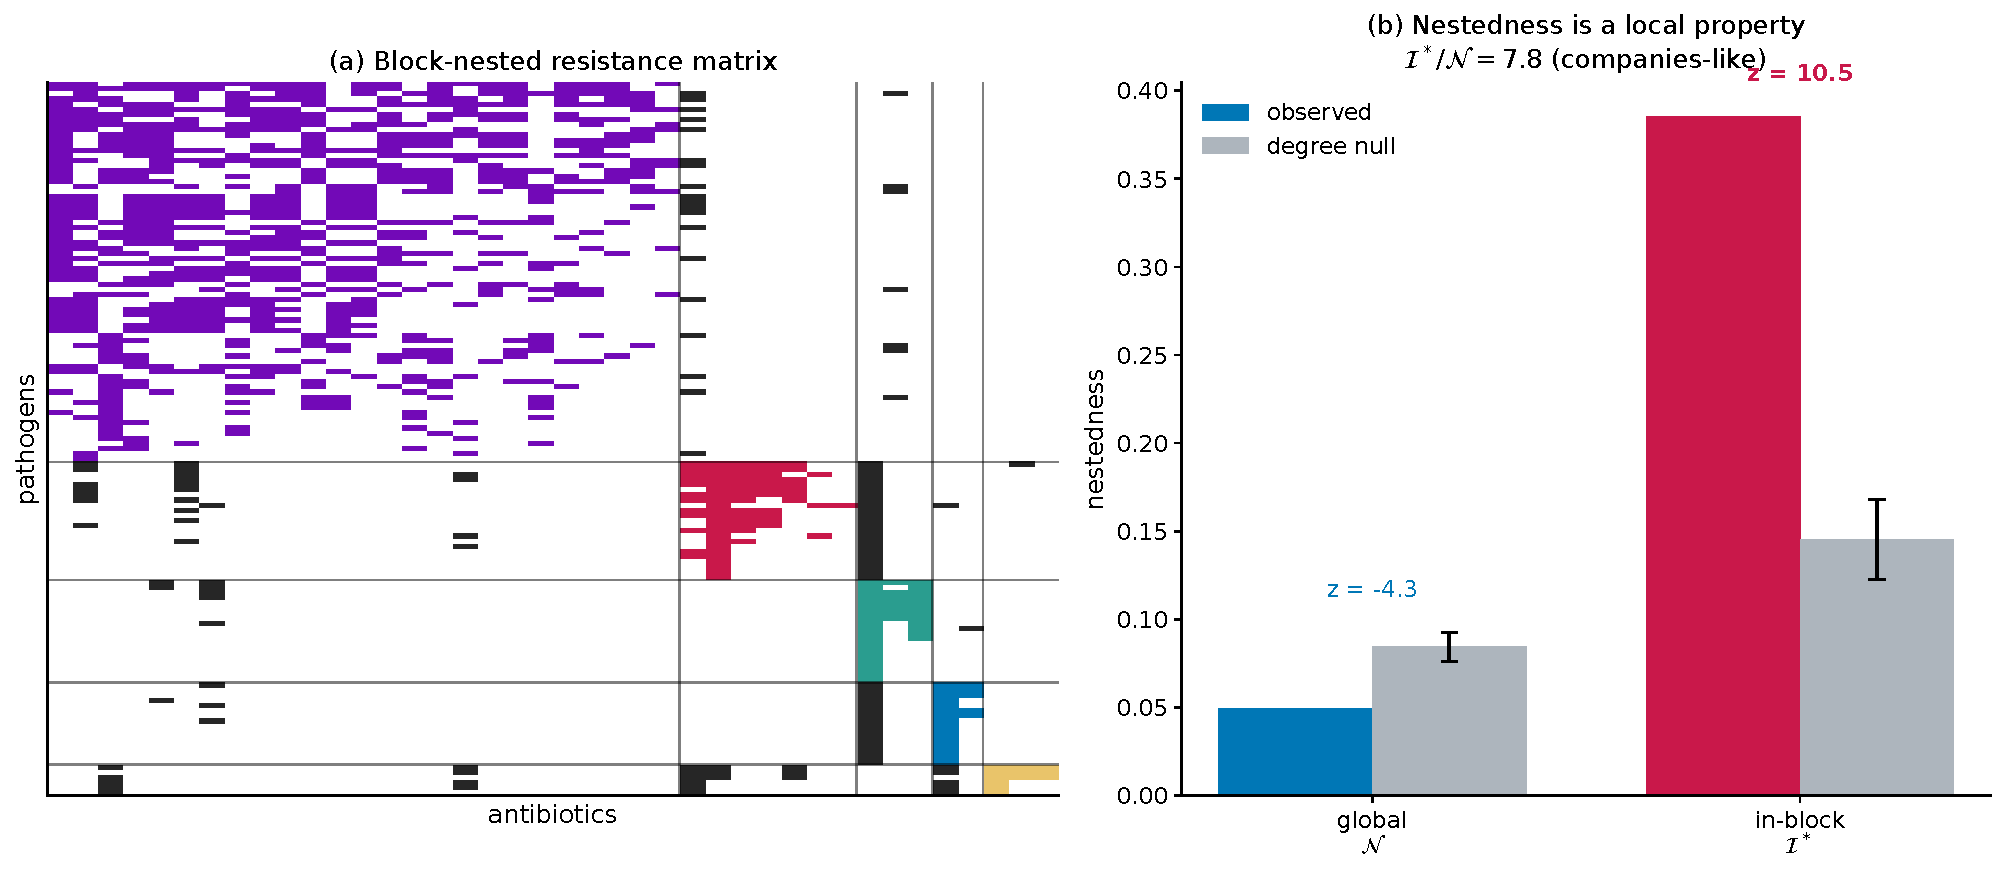
\includegraphics[width=0.94\textwidth]{figures/fig2_blocknested.pdf}
\caption{Global and local organisation of RCA-positive links. In (a), rows and columns are ordered by five spectral co-clusters and by degree within each cluster; coloured links lie within blocks and dark links connect blocks. Panel (b) compares global nestedness $\N$ and in-block nestedness $\I^*$ with the degree-corrected Bernoulli null implemented in the repository.}
\end{figure}

The co-clusters are therefore best interpreted as data-driven comparison contexts, not as predefined taxonomic or therapeutic categories. The result is also a property of the analysed surveillance matrix: because unobserved and observed RCA-negative cells both enter $M$ as zero, the structure reflects both positive comparative-resistance profiles and the testing and coverage pattern represented in ATLAS.

\newpage
\section*{Results (continued)}
\subsection*{Block-conditioned scores recover clinically recognisable ordering}
The modular result provides a diagnostic for FC. Applied to the full matrix, the nonlinear iteration collapses numerically onto one pathogen and one antibiotic: 138 of 139 global pathogen scores and 39 of 40 global antibiotic scores are below $10^{-10}$ after normalisation. Such a solution does not support a stable cross-module ranking. This behaviour follows from the nonlinear ``weakest-link'' update for antibiotic complexity: a positive link to a low-fitness pathogen strongly reduces complexity, and under repeated mean normalisation strongly separated components compete until one dominates the numerical scale. The collapse was diagnosed directly from the computed score distribution; it was not assumed from the nestedness result. Conditioning the calculation on the co-clusters avoids forcing unrelated profiles onto one axis.

Within blocks, antibiotic complexity increased across WHO AWaRe tiers (Spearman $\rho=0.5895$, $p=9.84\times10^{-5}$; 38 antibiotics with available scores). This association was stronger than for global antibiotic complexity ($\rho=0.4667$, $p=0.0024$), and reached $\rho=0.6244$ ($p=8.49\times10^{-4}$) in the largest block. Taxa matching the ESKAPEE reference list (the ESKAPE grouping extended with \emph{E. coli}) had higher within-block pathogen fitness than other taxa: median standardised fitness was $1.044$ for 16 matching taxa and $-0.387$ for 107 others (one-sided Mann--Whitney $p=4.60\times10^{-6}$). Within-block scores were z-standardised before pooling: they describe relative position within a module, not an absolute resistance scale shared across modules.

These comparisons are useful because neither AWaRe nor ESKAPEE was used to build the network, define the blocks or fit the scores. Their agreement provides an external check that the local axes capture recognisable stewardship and priority structure. Such agreement is not guaranteed by node degree or clustering alone because the reference labels were withheld from the construction. It does not imply equivalence: AWaRe classifies antibiotics for stewardship, ESKAPEE denotes selected high-priority taxa, and FC measures only the topology of RCA-positive links in this dataset.

\begin{figure}[H]
\centering
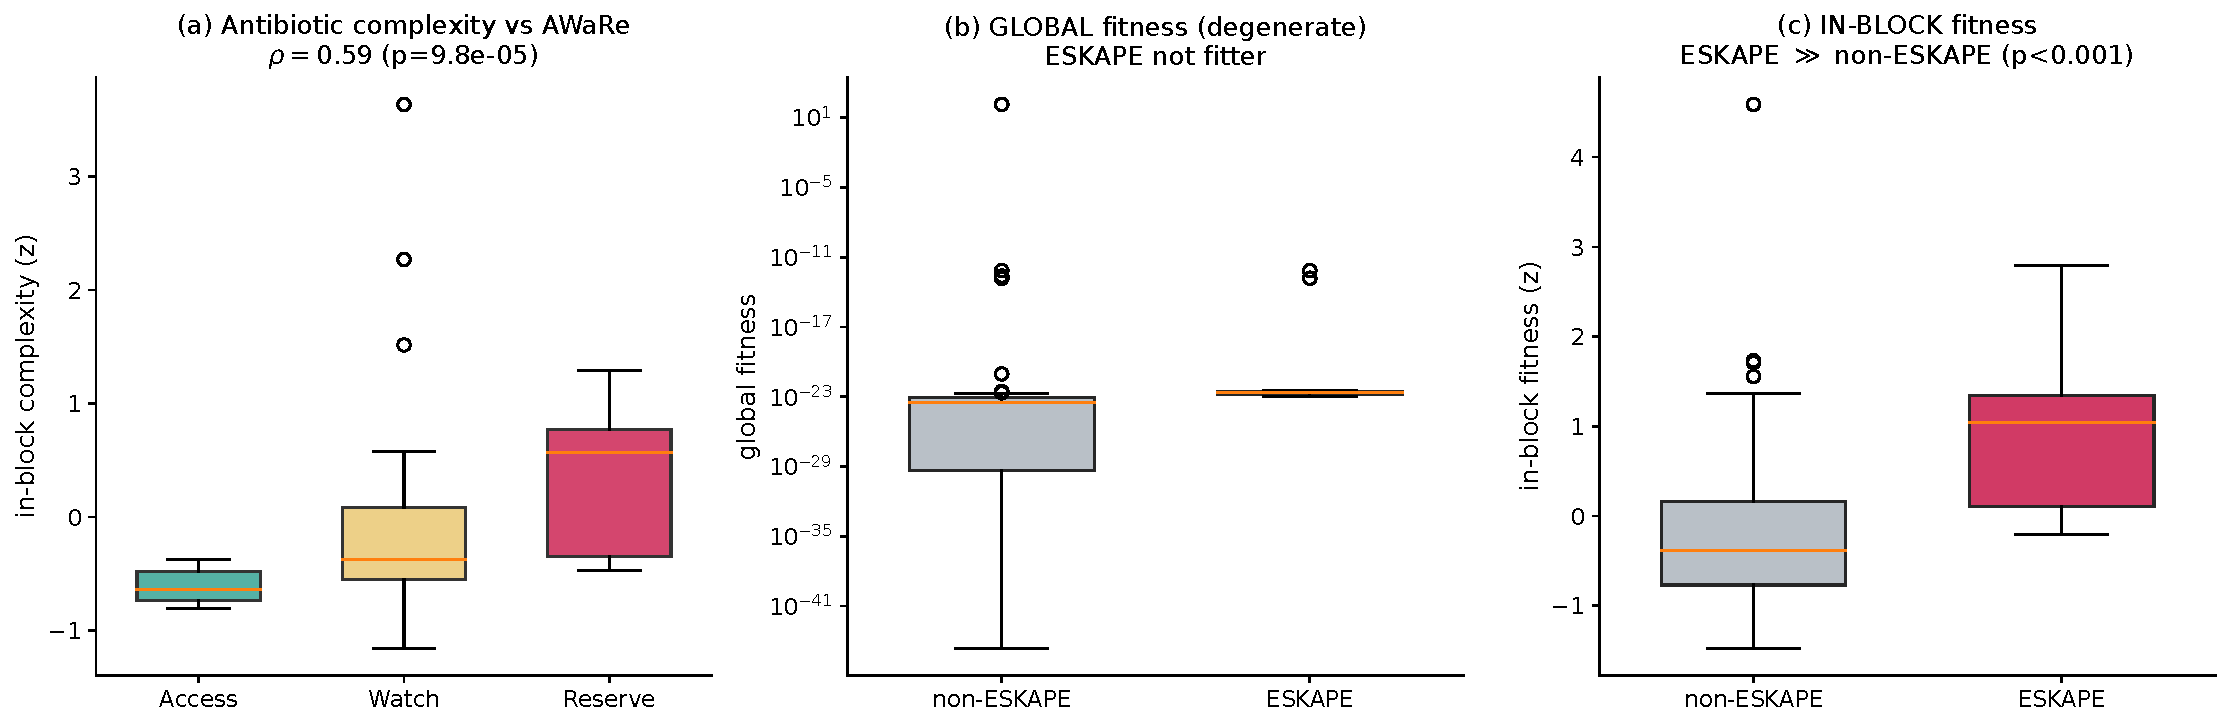
\includegraphics[width=0.96\textwidth]{figures/fig3_efc_validation.pdf}
\caption{External consistency of the network rankings. Panel (a) compares within-block antibiotic complexity with WHO AWaRe. Panel (b) shows the numerical collapse of the global FC solution, whereas (c) compares within-block pathogen fitness for taxa matching the ESKAPEE reference list and other taxa. Fitness is a mathematical network score, not evolutionary fitness.}
\end{figure}

The combination of the structural and validation results supports a local use of Economic Complexity: the informative comparison is not whether one pathogen is universally ``more resistant'' than another, but how broad and selective its revealed profile is relative to pathogens in the same co-resistance context.

\newpage
\section*{Results (continued)}
\subsection*{Network exposure prospectively prioritises next-year signals}
The rolling-origin back-test contained 1,839 eligible pathogen--antibiotic pair-years; 131 (7.12\%) were RCA-positive in the following year. Antibiotic-network exposure achieved a pooled AUC of $0.7076$, with origin-specific values from $0.6688$ to $0.7703$. Pathogen-network exposure achieved AUC $0.6283$, while the antibiotic RCA-link-ubiquity baseline was close to random ranking (AUC $0.5123$). An AUC of $0.7076$ means that a randomly selected future RCA-positive event received a higher exposure score than a randomly selected non-event in 70.76\% of comparisons; it is not classification accuracy or an individual probability.

The empirical gradient was also operationally interpretable. In sextiles of antibiotic-network exposure, 51 of 307 pairs (16.61\%) transitioned in the highest-exposure group, compared with 14 of 307 (4.56\%) in the lowest. Both projected-network scores exceeded the 200 node-label permutation comparisons reported by the pipeline run (empirical $p<0.005$). Per-antibiotic AUCs were highest for ceftazidime, gentamicin, meropenem, cefepime and ceftriaxone, but these subgroup estimates included only 5--9 events each and are therefore exploratory.

\begin{figure}[H]
\centering
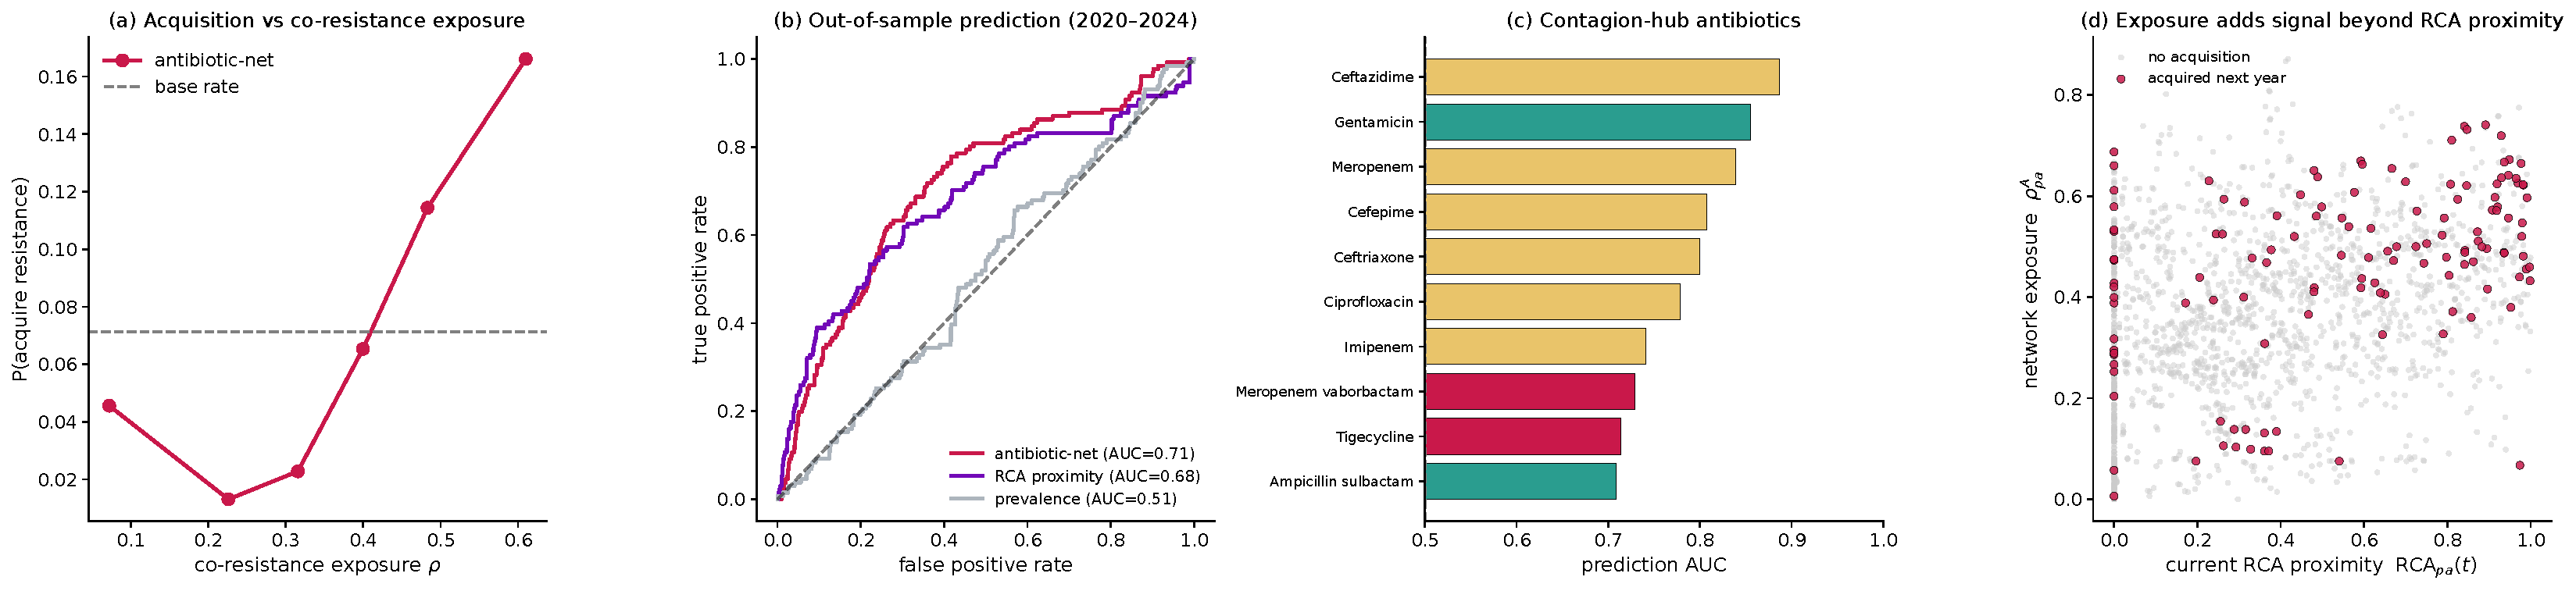
\includegraphics[width=0.62\textwidth]{figures/fig4_prediction.pdf}
\caption{Prospective prioritisation. Panel (a) shows the antibiotic relatedness network; (b) next-year event frequencies across exposure; (c) pooled rolling-origin ROC curves; and (d) performance by antibiotic. Raw co-occurrence drives prediction; degree normalisation affects only the layout in (a).}
\end{figure}

\section*{Impact of the work}
\begin{multicols}{2}
\small
The framework adds an interpretable relational layer to routine AMR surveillance. Its path is explicit---counts $\rightarrow r_{pa}\rightarrow\rca_{pa}\rightarrow M\rightarrow$ co-occurrence network $\rightarrow$ exposure ranking---so each prioritised pair can be traced to the observations, existing links and network neighbours that generated its score. This traceability is the practical distinction from a black-box forecast: the score itself is also its explanation. The reported ranking requires no fitted multivariable classifier and can be updated whenever new counts arrive. The repository provides the deterministic script, reference mappings, output tables, figures and a prototype dashboard. These outputs could support review, targeted testing or confirmatory analysis; they are not treatment recommendations.

The workflow can also address temporal and geographical heterogeneity. Isolate-level data can be filtered to a time period, country, region or continent, after which resistance fractions, RCA marginals, blocks and networks must be recomputed within that subset. Temporal re-estimation is demonstrated here. Geographic re-estimation is a deployment opportunity, not a reported result, because the committed downstream table is pooled across countries.

Interpretation remains bounded by the surveillance universe. RCA is relative rather than absolute; ATLAS sampling and testing are not population-random; and the implemented zero combines observed RCA-negative with insufficiently observed pairs. Five clusters are fixed, the nestedness null is only degree-corrected in expectation, and AWaRe/ESKAPEE provide external consistency rather than clinical validation. AUC measures ranking rather than calibrated risk, and the analysis does not establish causal acquisition, transmission, treatment failure or clinical outcome. Within these limits, the method offers a simple and reproducible route from surveillance counts to prospective prioritisation.
\end{multicols}

\newpage
\begin{thebibliography}{9}\small
\bibitem{atlas} Pfizer ATLAS antimicrobial surveillance programme, accessed through the Vivli AMR Register, 2004--2024. Vivli AMR Register: \url{https://amr.vivli.org/}.
\bibitem{hidalgo2009} Hidalgo CA, Hausmann R. The building blocks of economic complexity. \emph{Proc Natl Acad Sci USA}. 2009;106:10570--10575.
\bibitem{tacchella2012} Tacchella A, Cristelli M, Caldarelli G, Gabrielli A, Pietronero L. A new metrics for countries' fitness and products' complexity. \emph{Sci Rep}. 2012;2:723.
\bibitem{soleribalta2018} Sol\'e-Ribalta A, Tessone CJ, Mariani MS, Borge-Holthoefer J. Revealing in-block nestedness: detection and benchmarking. \emph{Phys Rev E}. 2018;97:062302.
\bibitem{laudati2023} Laudati D, Mariani MS, Pietronero L, Zaccaria A. The different structure of economic ecosystems at the scales of companies and countries. \emph{J Phys Complexity}. 2023;4:025011.
\bibitem{dhillon2001} Dhillon IS. Co-clustering documents and words using bipartite spectral graph partitioning. In: \emph{Proceedings of KDD}; 2001:269--274.
\bibitem{aware} World Health Organization. \emph{AWaRe classification of antibiotics for evaluation and monitoring of use, 2023}. WHO/MHP/HPS/EML/2023.04.
\bibitem{rice2008} Rice LB. Federal funding for the study of antimicrobial resistance in nosocomial pathogens: no ESKAPE. \emph{J Infect Dis}. 2008;197:1079--1081.
\end{thebibliography}

\end{document}
